
%% bare_jrnl.tex
%% V1.3
%% 2007/01/11
%% by Michael Shell
%% see http://www.michaelshell.org/
%% for current contact information.
%%
%% This is a skeleton file demonstrating the use of IEEEtran.cls
%% (requires IEEEtran.cls version 1.7 or later) with an IEEE journal paper.
%%
%% Support sites:
%% http://www.michaelshell.org/tex/ieeetran/
%% http://www.ctan.org/tex-archive/macros/latex/contrib/IEEEtran/
%% and
%% http://www.ieee.org/



% *** Authors should verify (and, if needed, correct) their LaTeX system  ***
% *** with the testflow diagnostic prior to trusting their LaTeX platform ***
% *** with production work. IEEE's font choices can trigger bugs that do  ***
% *** not appear when using other class files.                            ***
% The testflow support page is at:
% http://www.michaelshell.org/tex/testflow/


%%*************************************************************************
%% Legal Notice:
%% This code is offered as-is without any warranty either expressed or
%% implied; without even the implied warranty of MERCHANTABILITY or
%% FITNESS FOR A PARTICULAR PURPOSE! 
%% User assumes all risk.
%% In no event shall IEEE or any contributor to this code be liable for
%% any damages or losses, including, but not limited to, incidental,
%% consequential, or any other damages, resulting from the use or misuse
%% of any information contained here.
%%
%% All comments are the opinions of their respective authors and are not
%% necessarily endorsed by the IEEE.
%%
%% This work is distributed under the LaTeX Project Public License (LPPL)
%% ( http://www.latex-project.org/ ) version 1.3, and may be freely used,
%% distributed and modified. A copy of the LPPL, version 1.3, is included
%% in the base LaTeX documentation of all distributions of LaTeX released
%% 2003/12/01 or later.
%% Retain all contribution notices and credits.
%% ** Modified files should be clearly indicated as such, including  **
%% ** renaming them and changing author support contact information. **
%%
%% File list of work: IEEEtran.cls, IEEEtran_HOWTO.pdf, bare_adv.tex,
%%                    bare_conf.tex, bare_jrnl.tex, bare_jrnl_compsoc.tex
%%*************************************************************************

% Note that the a4paper option is mainly intended so that authors in
% countries using A4 can easily print to A4 and see how their papers will
% look in print - the typesetting of the document will not typically be
% affected with changes in paper size (but the bottom and side margins will).
% Use the testflow package mentioned above to verify correct handling of
% both paper sizes by the user's LaTeX system.
%
% Also note that the "draftcls" or "draftclsnofoot", not "draft", option
% should be used if it is desired that the figures are to be displayed in
% draft mode.
%
\documentclass[journal]{IEEEtran}
%\usepackage[spanish]{babel}
%
% If IEEEtran.cls has not been installed into the LaTeX system files,
% manually specify the path to it like:
% \documentclass[journal]{../sty/IEEEtran}





% Some very useful LaTeX packages include:
% (uncomment the ones you want to load)


% *** MISC UTILITY PACKAGES ***
%
%\usepackage{ifpdf}
% Heiko Oberdiek's ifpdf.sty is very useful if you need conditional
% compilation based on whether the output is pdf or dvi.
% usage:
% \ifpdf
%   % pdf code
% \else
%   % dvi code
% \fi
% The latest version of ifpdf.sty can be obtained from:
% http://www.ctan.org/tex-archive/macros/latex/contrib/oberdiek/
% Also, note that IEEEtran.cls V1.7 and later provides a builtin
% \ifCLASSINFOpdf conditional that works the same way.
% When switching from latex to pdflatex and vice-versa, the compiler may
% have to be run twice to clear warning/error messages.






% *** CITATION PACKAGES ***
%
%\usepackage{cite}
% cite.sty was written by Donald Arseneau
% V1.6 and later of IEEEtran pre-defines the format of the cite.sty package
% \cite{} output to follow that of IEEE. Loading the cite package will
% result in citation numbers being automatically sorted and properly
% "compressed/ranged". e.g., [1], [9], [2], [7], [5], [6] without using
% cite.sty will become [1], [2], [5]--[7], [9] using cite.sty. cite.sty's
% \cite will automatically add leading space, if needed. Use cite.sty's
% noadjust option (cite.sty V3.8 and later) if you want to turn this off.
% cite.sty is already installed on most LaTeX systems. Be sure and use
% version 4.0 (2003-05-27) and later if using hyperref.sty. cite.sty does
% not currently provide for hyperlinked citations.
% The latest version can be obtained at:
% http://www.ctan.org/tex-archive/macros/latex/contrib/cite/
% The documentation is contained in the cite.sty file itself.






% *** GRAPHICS RELATED PACKAGES ***
%
\usepackage[pdftex]{graphicx}
\DeclareGraphicsExtensions{.pdf,.jpeg,.png}
\usepackage[center]{caption}
% \graphicspath{{../pdf/}{../jpeg/}}
\ifCLASSINFOpdf
\else
  % or other class option (dvipsone, dvipdf, if not using dvips). graphicx
  % will default to the driver specified in the system graphics.cfg if no
  % driver is specified.
  % \usepackage[dvips]{graphicx}
  % declare the path(s) where your graphic files are
  % \graphicspath{{../eps/}}
  % and their extensions so you won't have to specify these with
  % every instance of \includegraphics
  % \DeclareGraphicsExtensions{.eps}
\fi
% graphicx was written by David Carlisle and Sebastian Rahtz. It is
% required if you want graphics, photos, etc. graphicx.sty is already
% installed on most LaTeX systems. The latest version and documentation can
% be obtained at: 
% http://www.ctan.org/tex-archive/macros/latex/required/graphics/
% Another good source of documentation is "Using Imported Graphics in
% LaTeX2e" by Keith Reckdahl which can be found as epslatex.ps or
% epslatex.pdf at: http://www.ctan.org/tex-archive/info/
%
% latex, and pdflatex in dvi mode, support graphics in encapsulated
% postscript (.eps) format. pdflatex in pdf mode supports graphics
% in .pdf, .jpeg, .png and .mps (metapost) formats. Users should ensure
% that all non-photo figures use a vector format (.eps, .pdf, .mps) and
% not a bitmapped formats (.jpeg, .png). IEEE frowns on bitmapped formats
% which can result in "jaggedy"/blurry rendering of lines and letters as
% well as large increases in file sizes.
%
% You can find documentation about the pdfTeX application at:
% http://www.tug.org/applications/pdftex





% *** MATH PACKAGES ***
%
%\usepackage[cmex10]{amsmath}
% A popular package from the American Mathematical Society that provides
% many useful and powerful commands for dealing with mathematics. If using
% it, be sure to load this package with the cmex10 option to ensure that
% only type 1 fonts will utilized at all point sizes. Without this option,
% it is possible that some math symbols, particularly those within
% footnotes, will be rendered in bitmap form which will result in a
% document that can not be IEEE Xplore compliant!
%
% Also, note that the amsmath package sets \interdisplaylinepenalty to 10000
% thus preventing page breaks from occurring within multiline equations. Use:
%\interdisplaylinepenalty=2500
% after loading amsmath to restore such page breaks as IEEEtran.cls normally
% does. amsmath.sty is already installed on most LaTeX systems. The latest
% version and documentation can be obtained at:
% http://www.ctan.org/tex-archive/macros/latex/required/amslatex/math/





% *** SPECIALIZED LIST PACKAGES ***
%
%\usepackage{algorithmic}
% algorithmic.sty was written by Peter Williams and Rogerio Brito.
% This package provides an algorithmic environment fo describing algorithms.
% You can use the algorithmic environment in-text or within a figure
% environment to provide for a floating algorithm. Do NOT use the algorithm
% floating environment provided by algorithm.sty (by the same authors) or
% algorithm2e.sty (by Christophe Fiorio) as IEEE does not use dedicated
% algorithm float types and packages that provide these will not provide
% correct IEEE style captions. The latest version and documentation of
% algorithmic.sty can be obtained at:
% http://www.ctan.org/tex-archive/macros/latex/contrib/algorithms/
% There is also a support site at:
% http://algorithms.berlios.de/index.html
% Also of interest may be the (relatively newer and more customizable)
% algorithmicx.sty package by Szasz Janos:
% http://www.ctan.org/tex-archive/macros/latex/contrib/algorithmicx/




% *** ALIGNMENT PACKAGES ***
%
%\usepackage{array}
% Frank Mittelbach's and David Carlisle's array.sty patches and improves
% the standard LaTeX2e array and tabular environments to provide better
% appearance and additional user controls. As the default LaTeX2e table
% generation code is lacking to the point of almost being broken with
% respect to the quality of the end results, all users are strongly
% advised to use an enhanced (at the very least that provided by array.sty)
% set of table tools. array.sty is already installed on most systems. The
% latest version and documentation can be obtained at:
% http://www.ctan.org/tex-archive/macros/latex/required/tools/


%\usepackage{mdwmath}
%\usepackage{mdwtab}
% Also highly recommended is Mark Wooding's extremely powerful MDW tools,
% especially mdwmath.sty and mdwtab.sty which are used to format equations
% and tables, respectively. The MDWtools set is already installed on most
% LaTeX systems. The lastest version and documentation is available at:
% http://www.ctan.org/tex-archive/macros/latex/contrib/mdwtools/


% IEEEtran contains the IEEEeqnarray family of commands that can be used to
% generate multiline equations as well as matrices, tables, etc., of high
% quality.


%\usepackage{eqparbox}
% Also of notable interest is Scott Pakin's eqparbox package for creating
% (automatically sized) equal width boxes - aka "natural width parboxes".
% Available at:
% http://www.ctan.org/tex-archive/macros/latex/contrib/eqparbox/





% *** SUBFIGURE PACKAGES ***
%\usepackage[tight,footnotesize]{subfigure}
% subfigure.sty was written by Steven Douglas Cochran. This package makes it
% easy to put subfigures in your figures. e.g., "Figure 1a and 1b". For IEEE
% work, it is a good idea to load it with the tight package option to reduce
% the amount of white space around the subfigures. subfigure.sty is already
% installed on most LaTeX systems. The latest version and documentation can
% be obtained at:
% http://www.ctan.org/tex-archive/obsolete/macros/latex/contrib/subfigure/
% subfigure.sty has been superceeded by subfig.sty.



%\usepackage[caption=false]{caption}
%\usepackage[font=footnotesize]{subfig}
% subfig.sty, also written by Steven Douglas Cochran, is the modern
% replacement for subfigure.sty. However, subfig.sty requires and
% automatically loads Axel Sommerfeldt's caption.sty which will override
% IEEEtran.cls handling of captions and this will result in nonIEEE style
% figure/table captions. To prevent this problem, be sure and preload
% caption.sty with its "caption=false" package option. This is will preserve
% IEEEtran.cls handing of captions. Version 1.3 (2005/06/28) and later 
% (recommended due to many improvements over 1.2) of subfig.sty supports
% the caption=false option directly:
%\usepackage[caption=false,font=footnotesize]{subfig}
%
% The latest version and documentation can be obtained at:
% http://www.ctan.org/tex-archive/macros/latex/contrib/subfig/
% The latest version and documentation of caption.sty can be obtained at:
% http://www.ctan.org/tex-archive/macros/latex/contrib/caption/




% *** FLOAT PACKAGES ***
%
%\usepackage{fixltx2e}
% fixltx2e, the successor to the earlier fix2col.sty, was written by
% Frank Mittelbach and David Carlisle. This package corrects a few problems
% in the LaTeX2e kernel, the most notable of which is that in current
% LaTeX2e releases, the ordering of single and double column floats is not
% guaranteed to be preserved. Thus, an unpatched LaTeX2e can allow a
% single column figure to be placed prior to an earlier double column
% figure. The latest version and documentation can be found at:
% http://www.ctan.org/tex-archive/macros/latex/base/



%\usepackage{stfloats}
% stfloats.sty was written by Sigitas Tolusis. This package gives LaTeX2e
% the ability to do double column floats at the bottom of the page as well
% as the top. (e.g., "\begin{figure*}[!b]" is not normally possible in
% LaTeX2e). It also provides a command:
%\fnbelowfloat
% to enable the placement of footnotes below bottom floats (the standard
% LaTeX2e kernel puts them above bottom floats). This is an invasive package
% which rewrites many portions of the LaTeX2e float routines. It may not work
% with other packages that modify the LaTeX2e float routines. The latest
% version and documentation can be obtained at:
% http://www.ctan.org/tex-archive/macros/latex/contrib/sttools/
% Documentation is contained in the stfloats.sty comments as well as in the
% presfull.pdf file. Do not use the stfloats baselinefloat ability as IEEE
% does not allow \baselineskip to stretch. Authors submitting work to the
% IEEE should note that IEEE rarely uses double column equations and
% that authors should try to avoid such use. Do not be tempted to use the
% cuted.sty or midfloat.sty packages (also by Sigitas Tolusis) as IEEE does
% not format its papers in such ways.


%\ifCLASSOPTIONcaptionsoff
%  \usepackage[nomarkers]{endfloat}
% \let\MYoriglatexcaption\caption
% \renewcommand{\caption}[2][\relax]{\MYoriglatexcaption[#2]{#2}}
%\fi
% endfloat.sty was written by James Darrell McCauley and Jeff Goldberg.
% This package may be useful when used in conjunction with IEEEtran.cls'
% captionsoff option. Some IEEE journals/societies require that submissions
% have lists of figures/tables at the end of the paper and that
% figures/tables without any captions are placed on a page by themselves at
% the end of the document. If needed, the draftcls IEEEtran class option or
% \CLASSINPUTbaselinestretch interface can be used to increase the line
% spacing as well. Be sure and use the nomarkers option of endfloat to
% prevent endfloat from "marking" where the figures would have been placed
% in the text. The two hack lines of code above are a slight modification of
% that suggested by in the endfloat docs (section 8.3.1) to ensure that
% the full captions always appear in the list of figures/tables - even if
% the user used the short optional argument of \caption[]{}.
% IEEE papers do not typically make use of \caption[]'s optional argument,
% so this should not be an issue. A similar trick can be used to disable
% captions of packages such as subfig.sty that lack options to turn off
% the subcaptions:
% For subfig.sty:
% \let\MYorigsubfloat\subfloat
% \renewcommand{\subfloat}[2][\relax]{\MYorigsubfloat[]{#2}}
% For subfigure.sty:
% \let\MYorigsubfigure\subfigure
% \renewcommand{\subfigure}[2][\relax]{\MYorigsubfigure[]{#2}}
% However, the above trick will not work if both optional arguments of
% the \subfloat/subfig command are used. Furthermore, there needs to be a
% description of each subfigure *somewhere* and endfloat does not add
% subfigure captions to its list of figures. Thus, the best approach is to
% avoid the use of subfigure captions (many IEEE journals avoid them anyway)
% and instead reference/explain all the subfigures within the main caption.
% The latest version of endfloat.sty and its documentation can obtained at:
% http://www.ctan.org/tex-archive/macros/latex/contrib/endfloat/
%
% The IEEEtran \ifCLASSOPTIONcaptionsoff conditional can also be used
% later in the document, say, to conditionally put the References on a 
% page by themselves.





% *** PDF, URL AND HYPERLINK PACKAGES ***
%
%\usepackage{url}
% url.sty was written by Donald Arseneau. It provides better support for
% handling and breaking URLs. url.sty is already installed on most LaTeX
% systems. The latest version can be obtained at:
% http://www.ctan.org/tex-archive/macros/latex/contrib/misc/
% Read the url.sty source comments for usage information. Basically,
% \url{my_url_here}.





% *** Do not adjust lengths that control margins, column widths, etc. ***
% *** Do not use packages that alter fonts (such as pslatex).         ***
% There should be no need to do such things with IEEEtran.cls V1.6 and later.
% (Unless specifically asked to do so by the journal or conference you plan
% to submit to, of course. )


% correct bad hyphenation here
%\hyphenation{op-tical net-works semi-conduc-tor}


\begin{document}
%
% paper title
% can use linebreaks \\ within to get better formatting as desired
\title{Algoritmo de evasi\'on de obst\'aculos en tiempo real basado en visi\'on est\'ereo}
%
%
% author names and IEEE memberships
% note positions of commas and nonbreaking spaces ( ~ ) LaTeX will not break
% a structure at a ~ so this keeps an author's name from being broken across
% two lines.
% use \thanks{} to gain access to the first footnote area
% a separate \thanks must be used for each paragraph as LaTeX2e's \thanks
% was not built to handle multiple paragraphs
%

\author{Taih\'u Pire,~\IEEEmembership{Member,~FCEyN-UBA,}
        Sergio Gonz\'alez,~\IEEEmembership{Fellow,~FCEyN-UBA,}
        Emiliano Gonz\'alez,~\IEEEmembership{Life~Fellow,~FCEyN-UBA}
        Ra\'ul Benniti,~\IEEEmembership{Fellow,~FCEyN-UBA,}% <-this % stops a space
        }
%\thanks{M. Shell is with the Department
%of Electrical and Computer Engineering, Georgia Institute of Technology, Atlanta,
%GA, 30332 USA e-mail: (see http://www.michaelshell.org/contact.html).}% <-this % stops a space
%\thanks{J. Doe and J. Doe are with Anonymous University.}% <-this % stops a space
%\thanks{Manuscript received April 19, 2005; revised January 11, 2007.}}

% note the % following the last \IEEEmembership and also \thanks - 
% these prevent an unwanted space from occurring between the last author name
% and the end of the author line. i.e., if you had this:
% 
% \author{....lastname \thanks{...} \thanks{...} }
%                     ^------------^------------^----Do not want these spaces!
%
% a space would be appended to the last name and could cause every name on that
% line to be shifted left slightly. This is one of those "LaTeX things". For
% instance, "\textbf{A} \textbf{B}" will typeset as "A B" not "AB". To get
% "AB" then you have to do: "\textbf{A}\textbf{B}"
% \thanks is no different in this regard, so shield the last } of each \thanks
% that ends a line with a % and do not let a space in before the next \thanks.
% Spaces after \IEEEmembership other than the last one are OK (and needed) as
% you are supposed to have spaces between the names. For what it is worth,
% this is a minor point as most people would not even notice if the said evil
% space somehow managed to creep in.



% The paper headers
\markboth{Journal of \LaTeX\ Class Files,~Vol.~6, No.~1, January~2007}%
{Shell \MakeLowercase{\textit{et al.}}: Bare Demo of IEEEtran.cls for Journals}
% The only time the second header will appear is for the odd numbered pages
% after the title page when using the twoside option.
% 
% *** Note that you probably will NOT want to include the author's ***
% *** name in the headers of peer review papers.                   ***
% You can use \ifCLASSOPTIONpeerreview for conditional compilation here if
% you desire.




% If you want to put a publisher's ID mark on the page you can do it like
% this:
%\IEEEpubid{0000--0000/00\$00.00~\copyright~2007 IEEE}
% Remember, if you use this you must call \IEEEpubidadjcol in the second
% column for its text to clear the IEEEpubid mark.



% use for special paper notices
%\IEEEspecialpapernotice{(Invited Paper)}




% make the title area
\maketitle


\begin{abstract}
En el presente trabajo se evaluar\'a un algoritmo de evasi\'on de obst\'aculos para navegaci\'on aut\'onoma de robots basado en mapas de profundidad. Aunque existen diversas tecnolog\'ias que permiten generar dichos mapas, los m\'etodos de visi\'on est\'ereo que generan mapas de disparidad han ganado relevancia en los \'ultimos a\~nos debido a la accesibilidad de los elementos de hardware necesarios tanto como para obtener la informaci\'on sobre el entorno inmediato, como para procesarla. Se considerar\'an dos partes principales en el desarrollo propuesto: en primer lugar, se utilizar\'an las librer\'ias open source de procesamiento gr\'afico OpenCV y Libelas para, a partir de las im\'agenes provistas por una c\'amara \'estereo, generar mapas de disparidad de los que se pueda deducir informaci\'on relevante a la distancia de los objetos dentro de la ventana de visibilidad del robot; luego, se procesar\'an estos mapas para decidir si existe un obst\'aculo frente al robot y, de ser as\'i, divisar que acci\'on debe tomarse para evitarlo.
\end{abstract}
% IEEEtran.cls defaults to using nonbold math in the Abstract.
% This preserves the distinction between vectors and scalars. However,
% if the journal you are submitting to favors bold math in the abstract,
% then you can use LaTeX's standard command \boldmath at the very start
% of the abstract to achieve this. Many IEEE journals frown on math
% in the abstract anyway.

% Note that keywords are not normally used for peerreview papers.
\begin{IEEEkeywords}
IEEEtran, journal, \LaTeX, paper, template.
\end{IEEEkeywords}






% For peer review papers, you can put extra information on the cover
% page as needed:
% \ifCLASSOPTIONpeerreview
% \begin{center} \bfseries EDICS Category: 3-BBND \end{center}
% \fi
%
% For peerreview papers, this IEEEtran command inserts a page break and
% creates the second title. It will be ignored for other modes.
\IEEEpeerreviewmaketitle


\section{Introducci\'on}
%comentar el uso de un sistema de navegacion, basado en camaras stereo. justificando (barato, accesible, costo computacional)


En la \'ultima d\'ecada se ha dado un gran impulso al \'area de rob\'otica abocada a la navegaci\'on aut\'onoma de veh\'iculos. Dado que el campo de aplicaci\'on es diverso, abarcando desde sistemas tan cr\'iticos como la exploraci\'on de lugares inaccesibles para veh\'iculos tripulados, hasta sistemas tan sencillos como la realizaci\'on de tareas dom\'esticas aut\'onomas, se han desarrollados tecnologias de distinta complejidad y costo operativo. En especial, se ha hecho principal incapi\'e en los sistemas basados en visi\'on dado la variedad y el bajo costo que presentan las c\'amaras hoy en d\'ia.

En el presente informe se exhibe un algoritmo de evansi\'on de obst\'aculos basado \'unicamente en visi\'on est\'ereo para la navegaci\'on aut\'onoma de un robot. Visi\'on est\'ereo es una herramienta muy utilizada para la navegaci\'on aut\'onoma en los \'ultimos a\~nos debido al bajo costo de las c\'amaras y a la gran cantidad de informaci\'on que brindan. El software aqu\'i presentado para lograr la detecci\'on de obst\'aculos hace uso de una c\'amara est\'ereo permitiendo aproximar la distancia relativa en la que se encuentran los objetos con respecto a la c\'amara.
Cabe destacar, que dicho algoritmo puede ser adaptado a cualquier dispositivo que cuente con una c\'amara est\'ereo. En lo que aqu\'i refiere, se utiliz\'o la c\'amara est\'ereo \emph{Minoru}, y como plataforma de prueba el robot \emph{exabot} \cite{DPSC09}.

%Otra de las ventajas de utilizar visi\'on est\'ereo para la navegaci\'on aut\'onoma, es la posibilidad de crear mapas 3D del entorno, si bien aqu\'i no se

El documento esta estructurado de la siquienta manera: la secci\'on~\ref{sec:trabajajo_relacionado} introduce el estado del arte en sistemas de evasi\'on de obst\'aculos mediante el uso de visi\'on est\'ereo, la secci\'on~\ref{sec:hardware} detalla el hardware utilizado durante el desarrollo del algoritmo, la secci\'on~\ref{sec:pro_img} presenta las librer\'ias OpenCV y LIBELAS utilizadas para el procesamiento de im\'agenes y la generaci\'on de mapas de disparidad, la secci\'on~\ref{sec:heuristica} explica el algoritmo de evasi\'on de obst\'aculos propuesto, finalmente la secci\'on~\ref{sec:conclusiones} comenta algunas conclusiones y trabajo futuro.

\hfill 20 de Julio de 2012

\section{Trabajo Relacionado}
\label{sec:trabajajo_relacionado}

Una de las \'areas de mayor inter\'es dentro del campo de la rob\'otica es la de navegaci\'on aut\'onoma. Con el pasar del tiempo se han propuesto y creado diversos sistemas de navegaci\'on, que adem\'as de las metodolig\'ias algor\'itmicas utilizadas, se diferencian por la tecnolog\'ia utilizada para obtener la informaci\'on del mundo exterior que le permitir\'a realizar dicho desplazamiento.

Dentro de las tecnolog\'ias m\'as utilizadas, se encuentran entre otras:

\begin{itemize}
	\item La utilizaci\'on de {\bf c\'amaras de video}, que obtienen la informaci\'on en forma de im\'agenes. Los m\'etodos mas populares, utilizan una c\'amara (visi\'on monocular) o dos c\'amaras (visi\'on est\'ereo).
	
	\item La utilizaci\'on de sensores como por ejemplo {\bf sonares} o {\bf l\'aser}, para detectar objetos pr\'oximos.
	
	\item Utilizar {\bf GPS} sumado a un mapa del terreno donde el robot se desplazar\'a.
\end{itemize}

Adem\'as ex\'isten m\'etodos, que combinan distintas tecnolog\'ias y pueden ser utilizados en problemas de localizaci\'on y mapeo \cite{KNG10}.

La utilización de c\'amaras est\'ereo en particular, puede ser utilizada para la detecc\'ion de elementos en el espacio por donde se desplaza el robot y de forma muy eficiente, dado que es posible calcular la profundidad relativa de los objetos en el \'area de visi\'on. Teniendo en cuenta lo anteriormente mencionado, el trabajo actual demuestra que es posible realizar un sistema de evasi\'on de obstaculos, utilizando \'unicamente una c\'amara est\'ereo.

En el trabajo realizado por Kostavelis, Nalpantidis y Gasteratos \cite{KNG10}, se plantean diversas t\'ecnicas para mejorar el desempeño en la tarea de evasi\'on de obst\'aculos. La primera de ellas, sugiere tomar la imagen y separarla en tres partes, una parte izquierda, una central y una derecha. Para cada una de las zonas mencionadas se calcula entonces el promedio de disparidad y luego se toma aquella con menor promedio, indicando la direcci\'on a tomar, asumiendo que dicha zona es la que contiene menor cantidad de obst\'aculos. Si bien pareciera ser una t\'ecnica efectiva, se puede mejorar solo agregando algunas restricciones a lo definido. Es cuando se plantea el segundo m\'etodo (siendo este una evoluc\'ion del primero). Teniendo la imagen dividida en tres zonas, primeramente se toma la parte central y se buscan los p\'ixels que tengan una disparidad mayor a cierto valor l\'imite (de ahora en adelante T), se realiza un conteo, de forma de calcular el porcentaje de pixels con disparidad alta en la zona y poder determinar si, frente a la c\'amara hay un obst\'aculo cercano. Para realizar dicha decisi\'on, se dispone de otro valor l\'imite sobre el promedio calculado y si este lo sobrepasa se considera que existe un objeto lo suficientemente cerca y es entonces cuando hay que esquivarlo. Una vez que se decide realizar una acci\'on evasiva, es necesario saber para que lado girar, es cuando entran entonces las otras partes de la imagen y se produce el movimiento para el lado que tenga el menor promedio de pixeles con disparidad alta.

\section{Hardware Utilizado}
% Descripcion del robot, descripcion de la minoru, explicacion (breve) de la calibracion (uso de toolbox calib)
\label{sec:hardware}


En este trabajo se utiliz\'o el robot {\bf Exabot}, dise�ado y fabricado en la facultad FCEyN-UBA, Argentina. Se trata de un veh\'iculo m\'ovil con cuatro ruedas, unidas por dos orugas, y dos motores, lo que permite movimientos con dos grados de libertad en el plano. Se configur\'o con una c\'amara est\'ereo y montaje para computadoras port\'atiles. La interfaz de comunicaci\'on con el mismo es v\'ia red, que se utiliza \'unicamente para enviar comandos.

\begin{figure}[ht]
	\begin{center}
		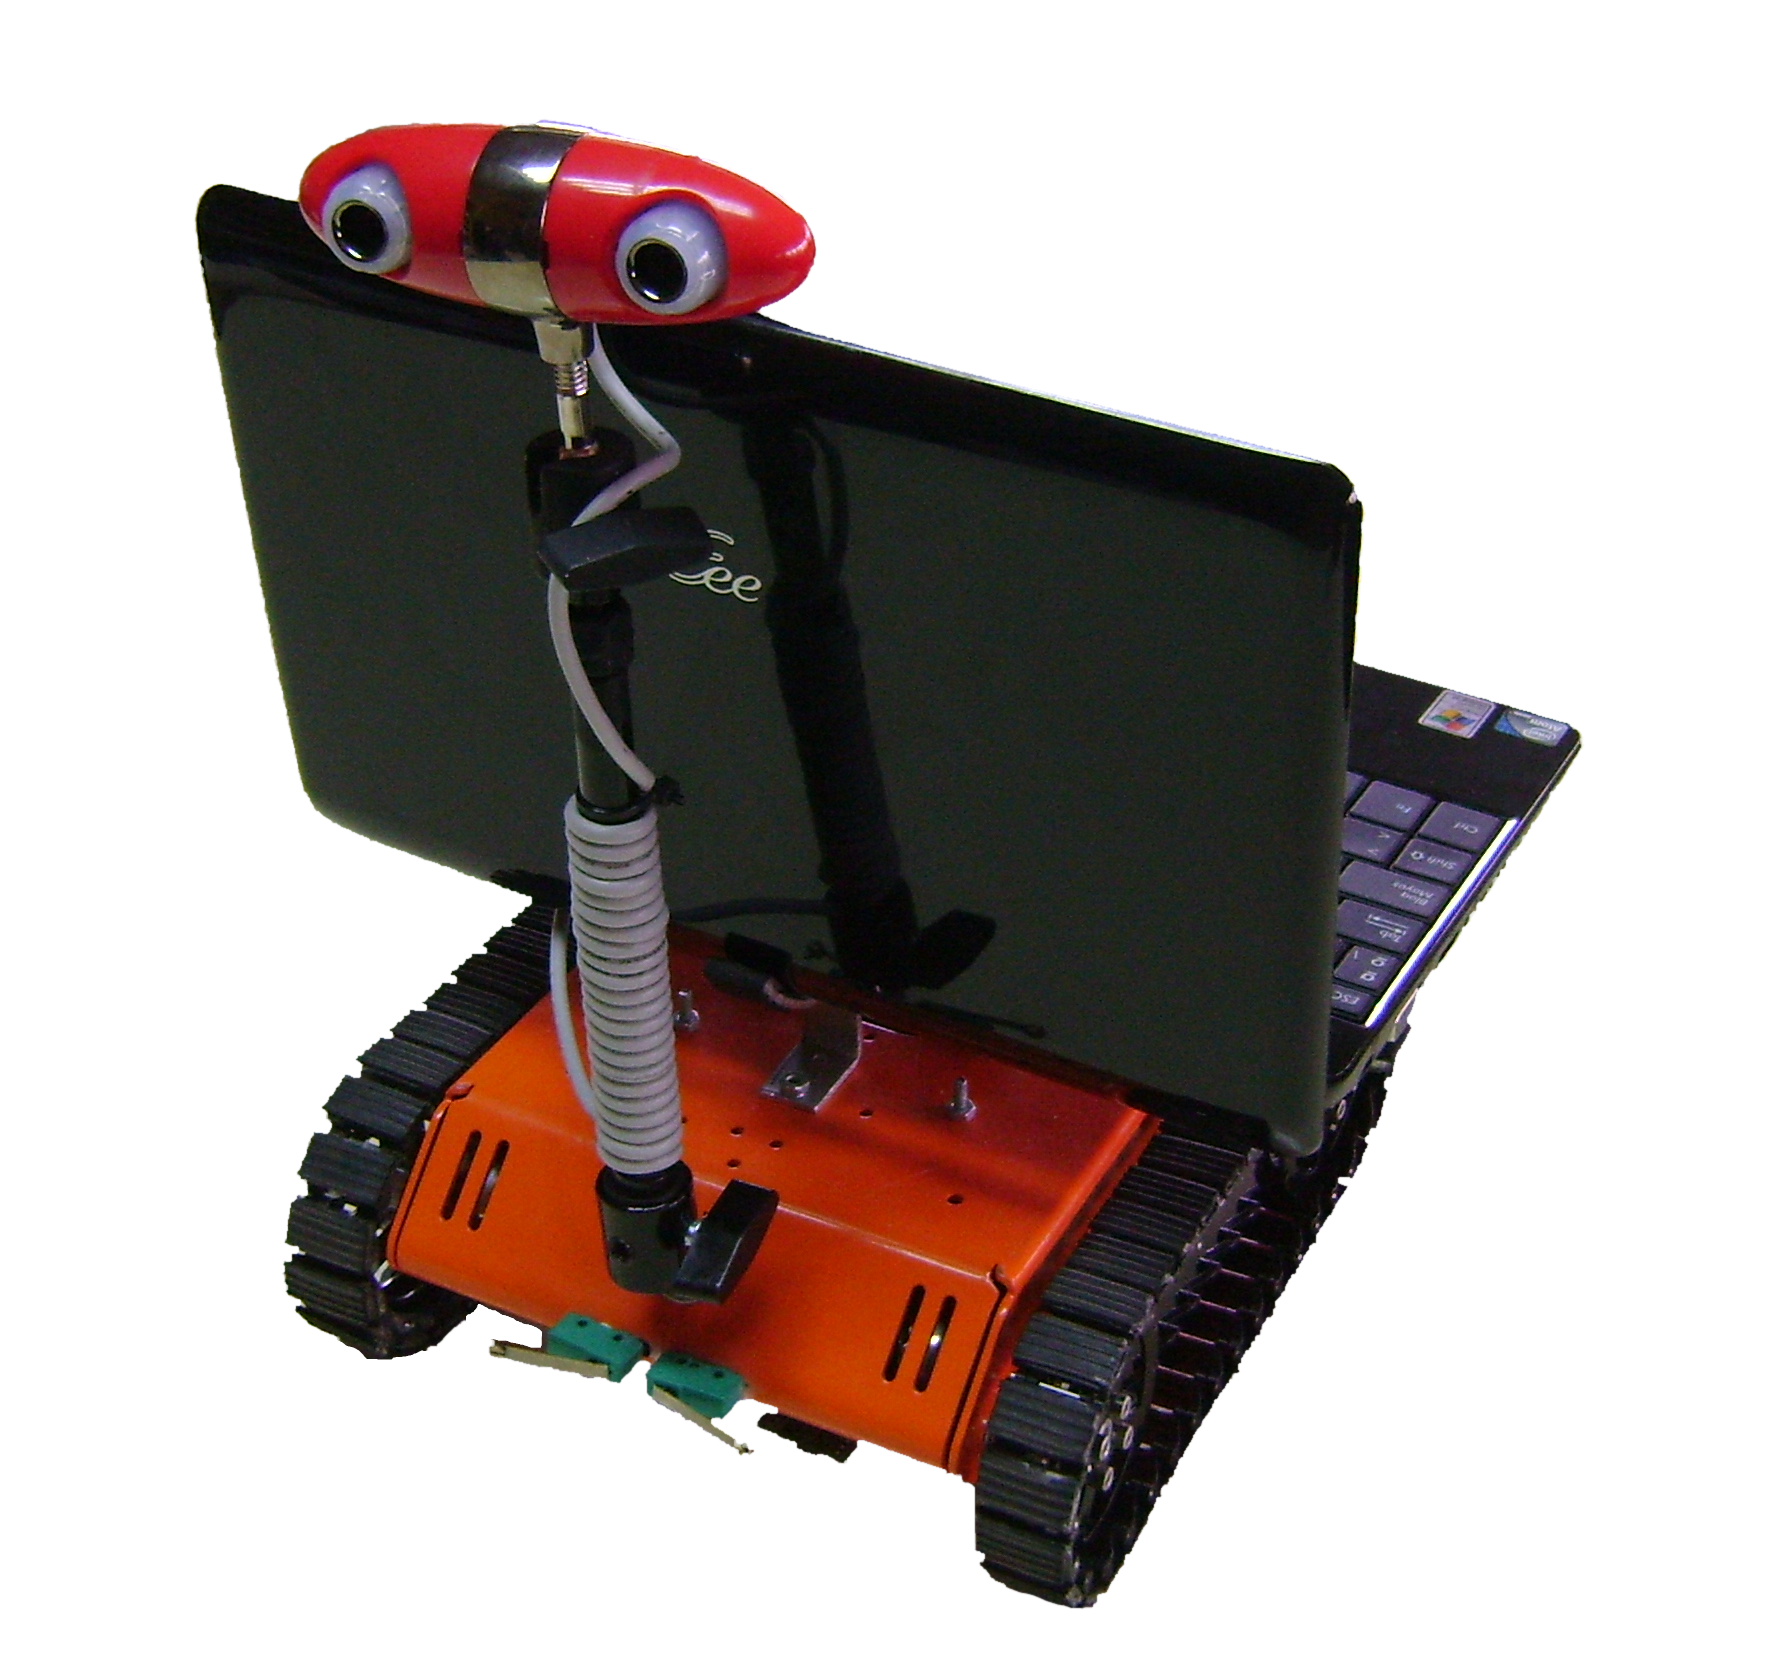
\includegraphics[width=6cm]{./images/exabot_04.png}
		\includegraphics[width=6cm]{./images/exabot_03.png}
		\caption{Configuraci\'on de Exabot utilizada}
	\end{center}
\end{figure}

El equipo de visi\'on est\'ereo montado en este trabajo es una c\'amara est\'ereo {\bf Minoru}. La misma se conecta v\'ia USB a la computadora port\'atil. Sus caracter\'isticas son las siguientes: 60 mm de base est\'ereo, USB 2.0, resoluciones desde 320x240 a 1280x480, 15~30fps, 1.5 W en modo operativo y 2 mW en modo suspendido. La resoluci\'on utilizada en este trabajo para las im\'agenes es de 640x480, capturadas a 15fps. Cabe aclarar que si bien la cantidad de im\'agenes disponibles por segundo es la mencionada anteriormente, las que realmente se procesan en general son menos, debido a la complejidad del algoritmo y el poder de c\'omputo del hardware.

En el contexto de algoritmos de Visi\'on, es mandatario calibrar las c\'amaras para poder identificar sus par\'ametros intr\'insecos (relativos a la c\'amara: distancia focal, punto principal, distorsi\'on radial) y extr\'insecos (de la c\'amara con respecto al mundo: rotaci\'on y traslaci\'on). Estos par\'ametros son luego utilizados para realizar las correctas transformaciones proyectivas a la imagen, que logran extraer informaci\'on de cada p\'ixel.

En este trabajo, utilizamos la matriz de calibraci\'on de cada c\'amara para rectificar las im\'agenes y calcular su mapa de disparidad correspondiente, como veremos en la secci\'on~\ref{sec:pro_img}.

La calibraci\'on de las c\'amaras se realiz\'o utilizando un paquete de MATLAB llamado {\bf Toolbox Calib} \cite{B00}. El producto de esta calibraci\'on est\'ereo es un archivo con los valores de los par\'ametros para ambas c\'amaras. Con este archivo se procede a generar otro con formato XML de una estructura en particular, que permite leerlo con la librer\'ia OpenCV.

\section{Procesamiento de las Ima\'genes}
\label{sec:pro_img}
%explicar la rectificacion y alineacion usando libelas y opencv y la generacion de mapas de disparidad

\begin{figure}[ht]
	\begin{center}
		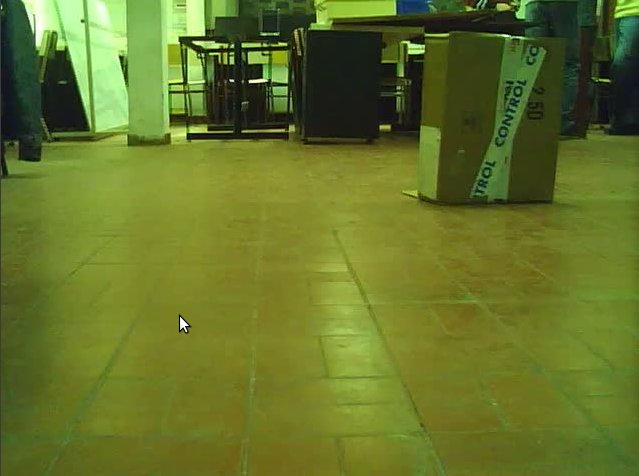
\includegraphics[width=6cm]{./images/original.jpg}
		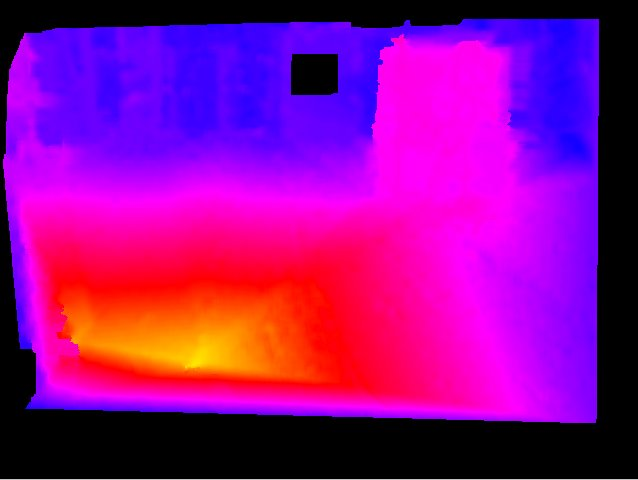
\includegraphics[width=6cm]{./images/disparidad.jpg}
		\caption{Captura de la c\'amara izquierda de la c\'amara Minoru (imagen superior) y su correspondiente mapa de disparidad (imagen inferiror).}
	\end{center}
\end{figure}

\section{Heur\'istica de Evasi\'on de Obst\'aculos}
%Explicacion de como se usa el mapa de disparidad (partiendo en 3 zonas etc.)(decir que solo se utiliza el mapa de un solo lado, izquierdo)
\label{sec:heuristica}

\section{Conclusiones}
%comentar que se pueden usar los dos mapas (de la parte derecha e izquierdas, etc)
\label{sec:conclusiones}
Se desarrollo un algoritmo para la evasi\'on de obst\'aculos basado en mapas de disparidad. Para el procesamiento de los mapas de profundida, se utilizaron las librer\'ias OpenCV (Open Source Computer Vision) que cuenta con funciones para visi\'on en computadora en tiempo real y LIBELAS (Library for Efficient LArge-scale Stereo Matching) espec\'ifica para la manipulaci\'on de imagenes est\'ereo de gran resoluci\'on. Por otro lado, se realizaron experimentos que verificaron el correcto comportamiento del m\'etodo implementado para la evasi\'on de obst\'aculos en tiempo real. Como trabajo futuro se podr\'ia integrar la informaci\'on provista por los mapas de disparidad resultantes de las imagenes izquierda y derecha logrando as\'i una mejor aproximaci\'on de profundidad. Adem\'as queda abierta la posibilidad de incorporar un m\'etodo de localizaci\'on y construcci\'on simult\'anea de Mapas, SLAM (por sus siglas en ingl\'es de Simultaneous localization and mapping) junto con un mecanismo de planeamiento de navegaci\'on.





\nocite{KNG10}
\nocite{G10}
\nocite{opencv}
\nocite{B00}
\nocite{H04}
\nocite{DPSC09}
\nocite{RH04}
\nocite{H09}

\bibliographystyle{unsrt}
\bibliography{biblio}

%\begin{thebibliography}{1}
%
%\bibitem{IEEEhowto:kopka}
%H.~Kopka and P.~W. Daly, \emph{A Guide to \LaTeX}, 3rd~ed.\hskip 1em plus
%  0.5em minus 0.4em\relax Harlow, England: Addison-Wesley, 1999.
%
%\end{thebibliography}

% that's all folks
\end{document}